\textbf{\underline{OZ 1 - Herhaling - Oefening 4:}}
\vspace{0.5cm}

\textbf{Elektrisch veld van een geladen staaf:} Een lading $ Q $ is uniform verdeeld over een staaf met lengte $ L $, zoals aangegeven op Figuur 1.2. De staaf is gelegen volgens de $ x $-as, met een uiteinde bij de oorsprong en het andere uiteinde ligt op punt $ x = L $. Bereken het elektrisch veld op het punt $ \left( L/2, D \right) $. Controleer je antwoord door de volgende limieten uit te rekenen: $ \lim_{ D \to \infty } \Vec{E} \left( L/2, D \right) $ en $ \lim_{ L \to \infty } \Vec{E} \left( L/2, D \right) $

\begin{figure}[h]
    \centering
    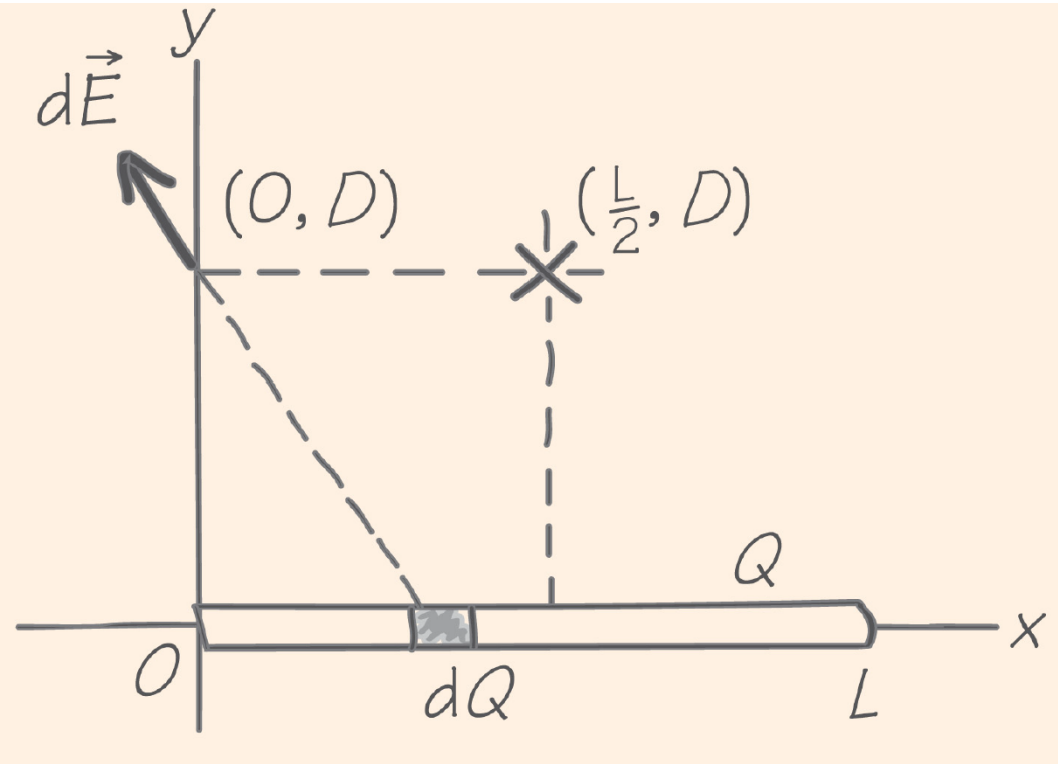
\includegraphics[width=4cm]{oz01/herhaling/resources/oef-4-opgave.png}
    
    \textbf{Figuur 1.2}
\end{figure}

\begin{description}[labelwidth=1.5cm, leftmargin=!]
    \item[Geg. :]   $ q = Q \cdot $ ; $ l = L \cdot m/s $ ; $ P(\frac{L}{2},D) $;
    \item[Gevr. :]  $ \vec{E_p}$;
    \item[Opl. :]   $ \vec{E_{p_y}} = 0  \Rightarrow \vec{E_p} = \vec{E_{p_x}} $
    
                    \textcolor{red}{TBD}
                    
\end{description}

\vspace{1cm}